\subsection{二面角}\label{subsec:1-14}

修筑水坝时,为了使永坝坚固耐久,必须使水坝面和水平面成适当的角度;
发射人造地球卫星时,也要根据需耍,使卫星的轨道平面和地球赤道平面成一定的角度(图 \ref{fig:ltjh-1-44})。
下面,我们来研究两个平面所成的角。

\begin{figure}[htbp]
    \centering
    \begin{minipage}[b]{7cm}
        \centering
        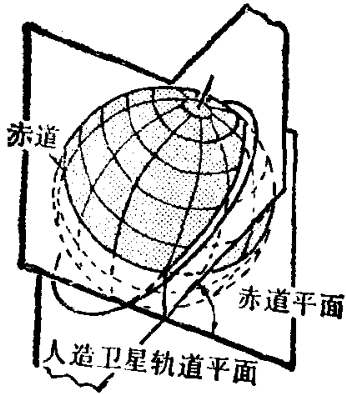
\includegraphics[width=5cm]{../pic/ltjh-ch1-44.png}
        \caption{}\label{fig:ltjh-1-44}
    \end{minipage}
    \qquad
    \begin{minipage}[b]{7cm}
        \centering
        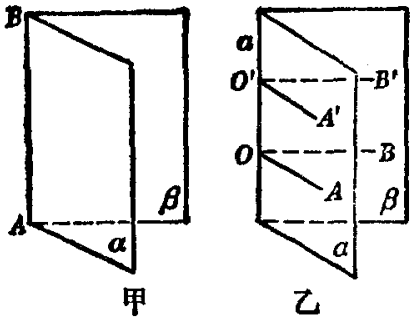
\includegraphics[width=6cm]{../pic/ltjh-ch1-45.png}
        \caption{}\label{fig:ltjh-1-45}
    \end{minipage}
\end{figure}

一个平面内的一条直线,把这个平面分成两部分,其中的每一部分都叫做\zhongdian{半平面}。
从一条直线出发的两个半平面所组成的图形叫做\zhongdian{二面角}(图 \ref{fig:ltjh-1-45} 甲)。
这条直线叫做\zhongdian{二面角的棱}。这两个半平面叫做\zhongdian{二面角的面}。

棱为 $AB$、面为 $\alpha$、$\beta$ 的二面角,记作二面角 $\alpha{-}AB{-}\beta$,
如果棱用 $a$ 表示,则记作二面角 $\alpha{-}a{-}\beta$。

如图 \ref{fig:ltjh-1-45} 乙,在二面角 $\alpha{-}a{-}\beta$ 的棱 $a$ 上任取一点 $O$,
在半平面 $\alpha$ 和 $\beta$ 内,从点 $O$ 分别作垂直于棱 $a$ 的射线 $OA$、$OB$,
射线 $OA$ 和 $OB$ 组成 $\angle AOB$。
在棱 $a$ 上另取任意一点 $O'$,按同样方法作 $\angle A'O'B'$。
因为 $OA$ 和 $O'A'$、$OB$ 和 $O'B'$ 都垂直于棱 $a$,
所以 $\angle AOB$ 和 $\angle A'O'B'$ 的两边分别平行且方向相同,
因此 $\angle AOB = \angle A'O'B'$。
可见, $\angle AOB$ 的大小与点 $O$ 在棱上的位置无关。

以二面角的棱上任意一点为端点,在两个面内分别作垂直于棱的两条射线,
这两条射线所成的角叫做\zhongdian{二面角的平面角}。

二面角的大小,可以用它的平面角来度量,二面角的平面角是几度,就说这个二面角是几度。

平面角是直角的二面角叫做\zhongdian{直二面角}。

木工用活动角尺测量工件的两个面所成的角时,实际上就是测量这两个面所成二面角的平面角(图 \ref{fig:ltjh-1-46})。
我国发射的第一颗人造地球卫是的倾角是 $68.5^\circ$,就是说卫星轨道平面与地球赤道平面所成的二面角的平面角是 $68.5^\circ$。

\begin{figure}[htbp]
    \centering
    \begin{minipage}[b]{7cm}
        \centering
        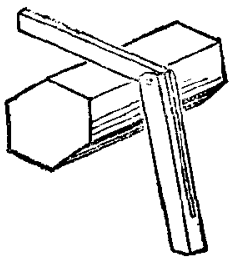
\includegraphics[width=4cm]{../pic/ltjh-ch1-46.png}
        \caption{}\label{fig:ltjh-1-46}
    \end{minipage}
    \qquad
    \begin{minipage}[b]{7cm}
        \centering
        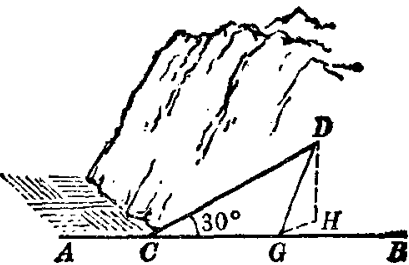
\includegraphics[width=6cm]{../pic/ltjh-ch1-47.png}
        \caption{}\label{fig:ltjh-1-47}
    \end{minipage}
\end{figure}

\liti[0] 如图 \ref{fig:ltjh-1-47},山坡的倾斜度(坡面与水平面所成二面角的度数)是 $60^\circ$,
山坡上有一条直道 $CD$,它和坡脚的水平线 $AB$ 的夹角是 $30^\circ$,沿这条路上山,行走 100 米后升高多少米?

\jie 已知 $CD = 100$ 米,设 $DH$ 垂直于过 $BC$ 的水平平面,垂足为$H$,
线段 $DH$ 的长度就是所求的高度。在平面 $DBC$内,
过点 $D$ 作 $DG \perp BC$,垂足是 $G$,连结 $GH$。

$\because$ \quad $DH \perp \text{平面}\;BCH$, $DG \perp BC$,

$\therefore$ \quad $GH \perp BC$。

因此, $\angle DGH$ 就是坡面 $DGC$ 和水平平面 $BCH$ 所成的二面角的平面角,
$\angle DGH = 60^\circ$。由此得
\begin{align*}
    DH &= DG \sin 60^\circ = CD \sin 30^\circ \sin 60^\circ \\
       &= 100 \sin 30^\circ \sin 60^\circ = 25\sqrt{3} \\
       &\approx 43.3 \; (\text{米})\juhao
\end{align*}

答:沿直道前进 100 米, 升高约 43.3 米。


\begin{lianxi}

\xiaoti{拿一张正三角形的纸片 $ABC$,以它的高 $AD$ 为折痕,折成一个二面角,指出这个二面角的面、棱、平面角。}

\xiaoti{一个平面垂直于二面角的棱,它和二面角的两个面的交线所成的角就是二面角的平面角。为什么?}

\xiaoti{教室相邻两面墙和天花板两两所成的二面角各有多少度?}

\xiaoti{在 $30^\circ$ 二面角的一个面内有一个点,它到另一个面的距离是 10 cm,求它到棱的距离。}

\end{lianxi}

